\chapter{Climate Finance}

\section*{Spend on building the resilience of poor people to the impacts of climate change and investing in low carbon development to avoid or reduce harmful greenhouse gases.}


\thispagestyle{empty}



\section{Results}
From 2016/17 to 2019/20, DFID spent \textbf{\pounds 2.9 billion} on building the resilience of poor people to the impacts of climate change and investing in low carbon development to avoid or prevent harmful greenhouse gases. %
This indicator contributes to the UK commitment to spend  \pounds  5.8 billion over five years on tackling climate change, of which DFID intends to spend \pounds3.6 billion. \\ %

\pounds 2.6 billion of DFID's spend on climate from 2016/17 to 2019/20 was through bilateral programmes by DFID's network of country offices, or by teams based in the UK whose programmes often operate across a range of countries. %
These programmes tackle climate change either as their main objective or alongside other development objectives such as economic development. \\ %

DFID, alongside the Department for Business, Energy and Industrial Strategy (BEIS) and the Department for Environment, Food and Rural Affairs (Defra), makes core contributions to specific multilateral organisations that tackle climate change, such as the Green Climate Fund and the Global Environment Facility. %
These organisations have greater reach across a broader range of countries and work with other donors to scale up climate finance faster and more effectively. %
DFID contributed \pounds 0.3 billion to climate multilaterals from 2016/17 to 2019/20. %

\begin{figure}[htbp]
  \centering
\begin{knitrout}
\definecolor{shadecolor}{rgb}{0.969, 0.969, 0.969}\color{fgcolor}
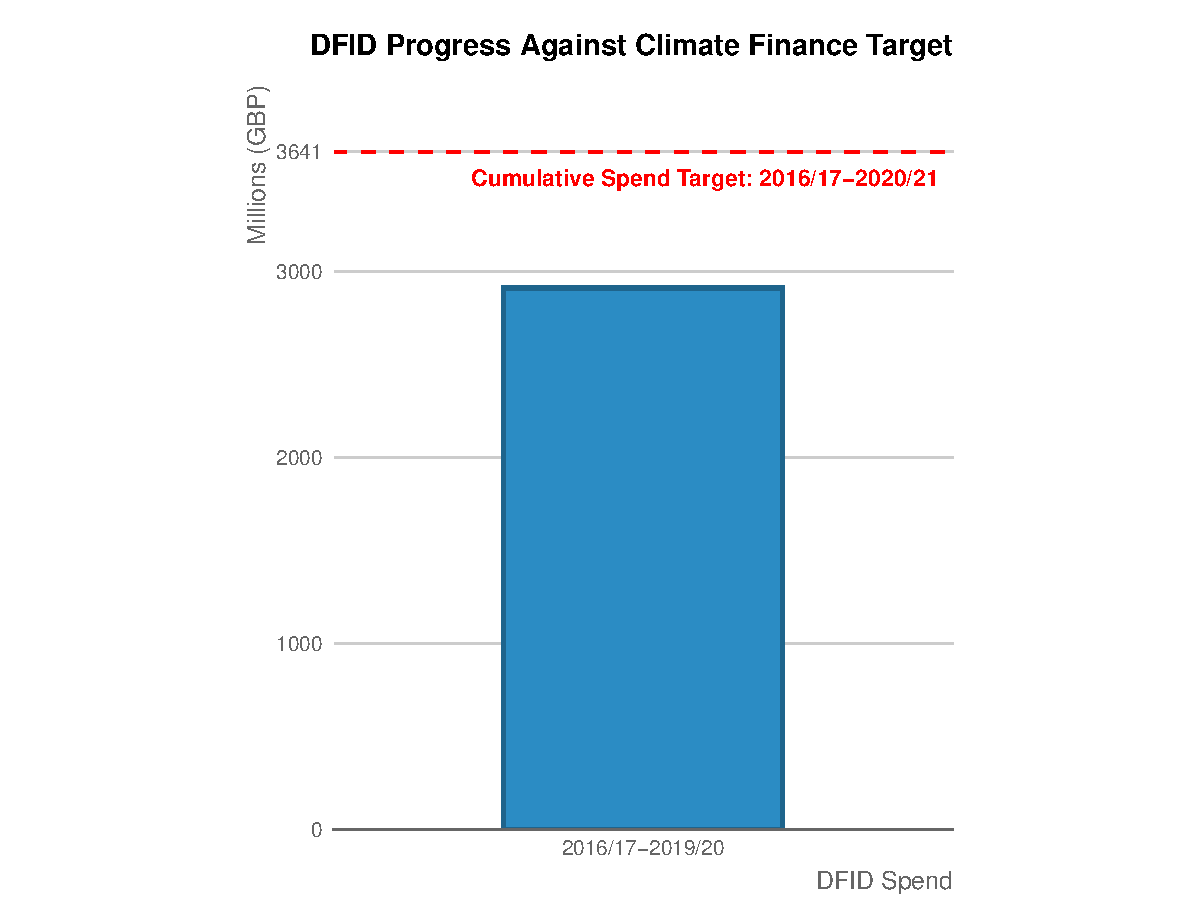
\includegraphics[width=0.8\textwidth]{figs/climate_spend_plot-1} 

\end{knitrout}
  \caption{DFID spend on climate finance from 2016/17 to 2019/2020 set against the cumulative spend target up to 2020/21 of \pounds 3,641 Million.}
  \label{fig:climate_spend_plot}
\end{figure}


\section{Context}

The World Bank estimates that an additional 100 million people could be in poverty by 2030 if climate change is not addressed. %
DFID recognises that poverty reduction and climate change are intrinsically linked and that action to tackle climate change must be embedded in DFID's work - in its engagement with partner countries, other donors and international organisations, and across its development portfolio - in order to drive sustainable decision-making in developing countries. \\%

The UK's International Climate Finance (ICF) aims to encourage transformational change in country resilience to climate change and disaster risk management, in sustainable management of natural resources such as forests, land and water and in access to clean energy and low carbon infrastructure. %
Alongside other developed countries, the UK has committed to jointly mobilise \$100 billion per year in climate finance to developing countries from public and private sources. %
DFID works jointly with BEIS and Defra on delivering this commitment using the UK aid budget. %

\subsection{Programmes using DFID Climate Finance}
Over 200 programmes contributed to DFID's climate finance spend during 2016/17-2019/20, using a range of instruments and covering a large number of sectors. %
Illustrative examples of this programming are noted below. \\%

DFID partnered with Germany to fund the Global Risk Financing Facility, which provides finance to support governments to use risk financing instruments, like insurance, to access more rapid finance in emergencies and to strengthen preparedness of local systems for disaster response and recovery. %
DFID also provided direct cash transfers to approximately 24,000 households living in arid and semi-arid areas of Kenya and has contributed to building a shock responsive system that now enables up to 374,000 households to be reached with cash in times of extreme drought emergencies. \\%

The Results Based Financing (RBF) for Low Carbon Energy Access programme has, since 2012 delivered energy access to at least 5.7 million people. %
A particularly successful model has been the Off-Grid Appliances RBF which has involved a bulk procurement incentive to distributors to deliver quality tested super- efficient off grid appliances like fridges, solar water pumps, and fans. This has led to the sale of over 250,000 efficient appliances in East Africa and Bangladesh through over 100 distributors to date. %
DFID support has enhanced Nepal's technical and negotiating capacity with a mix of home-grown expertise and international specialists to unlock investment in its hydro power export potential. %
Nepal is now set to double its current generation capacity, with a major \$1.2bn 900MW hydro power project currently under construction. \\%

DFID aims to drive a transformation towards sustainable management of these natural resources and protect the livelihoods of those who depend on them. %
DFID funding to the Forests Governance, Markets and Climate programme informed revision, in December 2019, of forest law in China to ban buying, transporting or processing illegally sourced timber, a major milestone in tackling illegal deforestation. \\%

In 2019, the UK (represented by DFID) held the developed country chair of the Green Climate Fund (GCF) Board. %
During this period, 32 projects worth US\$3.6 billion of GCF funding were approved by the GCF Board, including a solar rural electrification programme in Mali, directly benefiting 284,000 people and a clean cooking programme in Kenya and Senegal, directly benefiting over 11 million people. %
The GCF also completed its first replenishment, totalling US\$9.8 billion from 28 donors over the next four years, with the UK being the largest donor having doubled its contribution to \pounds 1.44 billion, funded by DFID and BEIS. \\%

Further information on UK International Climate Finance (ICF), including case studies, can be found on \href{https://www.gov.uk/guidance/international-climate-finance#our-portfolio-across-the-world}{GOV.UK} along with the \href{https://www.gov.uk/government/publications/uk-climate-finance-results}{latest UK Climate Finance Results}. %


\newpage
